%----------------------------------------
% Preamble to set up the document
%----------------------------------------
\documentclass{article}

% set up packages (you shouldn't need to touch this)
\usepackage{graphicx}  % required to insert images
\usepackage{hyperref}  % for hyperlinks
\usepackage[svgnames]{xcolor}  % to change hyperlink colors
\colorlet{linkcolour}{DarkBlue}
\hypersetup{colorlinks=true, linkcolor=linkcolour, citecolor=linkcolour, urlcolor=linkcolour,}

% Margins
\topmargin=-0.45in
\evensidemargin=0in
\oddsidemargin=0in
\textwidth=6.5in
\textheight=9.0in
\headsep=0.25in

% use a sans serif font
\renewcommand{\familydefault}{\sfdefault}

%----------------------------------------
% Step 1: Edit the lecture title
%----------------------------------------
\title{
Lecture 4: Counting at Scale \\  % Lecture title
Modeling Social Data, Spring 2017 \\   % Course title
Columbia University                    % School
}

%----------------------------------------
% Step 2: Edit your name and the date
%----------------------------------------
\author{Drew Johnston}                     % Scribe's name
\date{February 10th, 2017}                % Lecture date

\begin{document}

\maketitle


%----------------------------------------
% Step 3:
% Rename uni.tex to match your uni,
% edit the filename accordingly below,
% and put your notes in this file
%----------------------------------------
Lecture 4 can be broadly separated into two parts. The first is an expansion on methods for data preparation and cleaning, which we covered last week. The second expanded on our discussion of counting, talking about how to work on a substantially larger scale than before, using Hadoop and MapReduce.\\
\section{Data Preparation Part 2}
\subsection{Groupby and Vectorization}
We discussed groupby again, which is a function in R that we'll be using quite extensively. As a refresher, it allows you to break up a dataframe into groups, with each containing all the observations that share certain entries. For instance, let's say that you had a dataframe containing information about various people, with columns for gender, eye color, etc. Grouping the data by one of these columns breaks up the data according to the values in that column, so that you can consider the groups separately. For instance, grouping by eye color would create groups for each option--say, a group containing all of the blue-eyed people, another for the brown-eyed, etc. These could then easily be compared separately and concisely. Some important observations:\\
\begin{itemize}
\item Groupby is powerfully combined with the pipe command. For instance,\begin{verbatim}iris %>% group_by(Species) %>% summarize(count=n(),mean_length=mean(Sepal.Length))\end{verbatim} will compute the number of observations for each species and the mean sepal length within each species and display a summary table, as we saw in lecture.
\item The majority of important R verbs (like filter) will respect the groups within groupby and process accordingly.
\item The dataframe outputted by a groupby operation is modified, containing information about the categories. This makes it simple to perform grouped operations, but can make many operations give unexpected answers or perform poorly when this is not the functionality you are looking for. Be careful about when you are using the grouped and ungrouped tables!
\end{itemize}
\subsection{Pointers and Common Mistakes}
We then talked about some of the basics of R, and how to write effective and functional programs in it. Here are a few tips I thought were worth reemphasizing:\\
\begin{itemize}
\item In data processing, it's often handy to pass the results of one function into another in relatively complex ways. In R, you can do this in the standard way allowed by most programming languages, just nesting the functions within one another. This works fine, but can result in unreadable code if your pipeline is quite long. There is also the \%\textgreater\% function, which acts similarly to a Linux pipe. It normally just pipes the output of the function to its left to the first argument of the function on its right, but you can control the ordering. df \%\textgreater\% f() evaluates to f(df), df \%\textgreater\% f(x, .) evaluates to f(x, df).
\item Variable scoping can be a major source of confusion and unexpected behavior. A common error is creating local variables with the same name as columns in a dataframe, which can cause lots of frustration. Avoid this if at all possible!
\item Be sure to vectorize your functions if you're writing ones that ought to be applied to columns or rows of a dataframe! Functions designed to process a single item will be mighty confused when passed an array of such items. There's a built in vectorize function in R that you can pass your functions to in order to simplify this process.
\item If else statements can often be unsightly in R, especially when applied to vectors. There's an ifelse function that can be of help to you, functioning like a ternary operator. An example to which you can pass a vector of integers, which will provide a vector of strings as a result: \begin{verbatim}ifelse(a%%2==1,"odd","even") \end{verbatim}
\end{itemize}
\subsection{Joins}
R also includes functionality to allow for SQL-style joins between tables. This is quite important in the real world, as it allows you to combine data from a number of sources into one dataframe. There are several methods for joining data, depending on how you want data that appears in one data set but not the other to be treated. Here's a handy diagram from /r4ds.had.co.nz/diagrams/join-venn.png that I found helpful:\\ 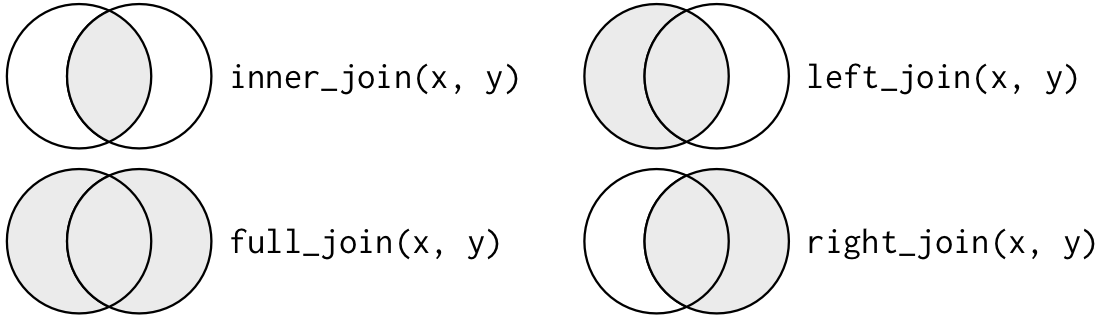
\includegraphics[width=\textwidth]{joins}\\
\begin{itemize}
\item There's a "by" argument that allows you to specify what columns in each dataframe you would like to join by comparing. For instance, $inner_join(df1, df2, by=c('firstname'='namefirst'))$ will perform an inner join on df1 and df2 by comparing column "firstname" in df1 to column "namefirst" in df2. R will try to guess how to perform the join if you don't include this argument, but it's best to keep it for the sake of clarity. 
\item R also has an anti-join command which can be used to see all of the values that are dropped when performing a join such as an inner join that does not preserve all of the information. This can be useful to ensure that you're not accidentally dropping lots of your information!
\item In this class, it's considered bad style to use right join. For the sake of clarity and consistency, it's preferred that you switch the order of the arguments and do a left join instead.
\subsection{Spread and Gather}
Spread and gather are two functions introduced by tidyr, which allow for you to "widen" or "lengthen" data by splitting up categorical values in rows into columns or by doing the reverse. This is very useful in plotting results. I found a neat and helpful example of spread on the internet (http://garrettgman.github.io/tidying/), which I'll reproduce here. It shows how you can turn the categories in a column full of categorical keys and a data column into two neatly organized columns.\\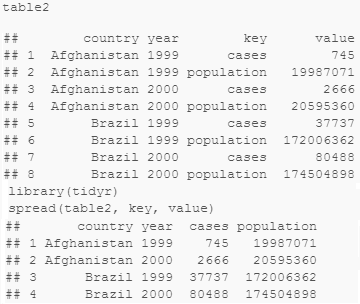
\includegraphics{spread}\\
Gather will do the reverse operation, converting specified columns into a categorical variable. It takes an additional argument, the indexes of the columns, to determine which columns should be converted into categories. Here's an example from the same site of gather in action: \\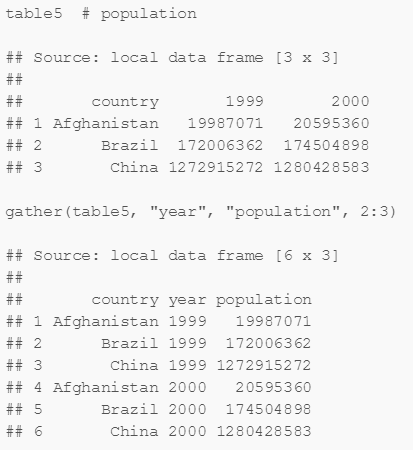
\includegraphics{gather}\\
\end{itemize}
\section{Intro to MapReduce and Hadoop}
\subsection{MapReduce}
MapReduce is a distributed solution to computational problems exceeding the processing power of a single machine. It has become extremely prominent within computer and data science in the last decade or so, as it is abstract enough to be applied as a framework to a large variety of parallelizable tasks. Essentially, it asks the programmer to implement a map function, which transforms the data into key-value pairs, as well as a reduce function, which lays out the computations that ought to be performed on each group. There's also a shuffle record that works behind the scenes, to collect all of the records with the same key together for the reduce function. This is advantageous if the processing takes a long time or if the disk access takes a long time, since both can be done in parallel. Some important points:\\
\begin{itemize}
\item Fault tolerance and synchronization are implemented under the hood, so the programmer doesn't need to worry about them when working on a new task.
\item MapReduce is designed to scale elegantly and transparently.
\item Strongest on tasks that are reading and bandwidth intensive.
\item Batch, offline, simple tasks are most frequently implemented in this way.
\item Some implementations can struggle when the tasks assigned to each computer take dramatically different amounts of time to finish.
\item MapReduce is useful for a great many tasks! But it's not always the right answer.
\end{itemize}
\subsection{Hadoop}
Hadoop is one of the most popular implementations of MapReduce principles. It's an open source program, which allows for existing code to be easily incorporated into a parallel structure. In many cases, it can save you from writing an entirely new program, since Hadoop as a streaming feature which allows you to just specify existing functions (like Unix builtins) as mappers and reducers. In the slides, there's an example where it's shown that a word counting program can be implemented in Hadoop without writing any Java code, using two lines of code and the Hadoop Streaming utility. Here's a great example taken from the slides, illustrating how easy it is to configure a program that would run locally to run in a distributed fashion:\\ 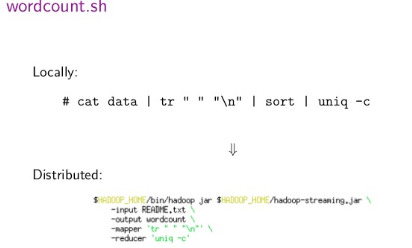
\includegraphics{hadoopstreaming}\\
Though using Hadoop and MapReduce concepts in traditional languages such as Python and Java is straightforward, there are also a number of high-level languages that were designed with bulk data processing in mind. Hadoop's team makes one called Pig that implements many common data analysis tasks as MapReduce jobs and is usable both on a single computer and in a larger production environment. We also mentioned Hive, another language for large scale data processing that is similar to SQL.

\end{document}

%%% Local Variables:
%%% mode: latex
%%% TeX-master: t
%%% End:
